\documentclass[hidelinks]{article}
\usepackage{graphicx} % Required for inserting images
% Language setting
% Replace `english' with e.g. `spanish' to change the document language
\usepackage[german]{babel}
\usepackage{longtable}

% Set page size and margins
% Replace `letterpaper' with `a4paper' for UK/EU standard size
%\usepackage[letterpaper,top=2.5cm,bottom=2cm,left=2.5cm,right=2.5cm,marginparwidth=1.75cm]{geometry}
\usepackage[a4paper,top=2cm,bottom=2cm,left=2.5cm,right=2.5cm,marginparwidth=1.75cm]{geometry}

% Useful packages
\usepackage{amsmath,amsthm}
\usepackage{comment}
\usepackage{enumerate}
\usepackage{fancyhdr}
\usepackage{xcolor}
\usepackage{inputenc}
\usepackage{float}
\usepackage[justification=centering]{caption}
\usepackage{csquotes}
\usepackage{tikz}
\usepackage{multicol}
\usepackage{amsmath,amssymb}
\usepackage{wrapfig}
\usepackage{notes2bib}
\PassOptionsToPackage{hyphens}{url}\usepackage{hyperref} % makes urls break
\hypersetup{
    colorlinks=true,
    linkcolor=blue,
    filecolor=magenta,
    urlcolor=cyan,
    pdftitle={Localic Caratheodory Extensions},
    pdfpagemode=FullScreen,
}
\usepackage{svg}
\usepackage{subcaption}

%---------- Lean Syntax Highlighting ----------
\usepackage{fontspec}
% switch to a monospace font supporting more Unicode characters
% \setmonofont{FreeMono}
\setmonofont{JetBrains Mono}
\usepackage{minted}
% instruct minted to use our local theorem.py
\newmintinline[lean]{lean}{bgcolor=white,fontsize=\small}
\newminted[leancode]{lean}{fontsize=\footnotesize,baselinestretch=1.2}
\usemintedstyle{tango}  % a nice, colorful theme


\usepackage[url=true,backend=biber]{biblatex}

% Command for marking things as leanok
\definecolor{darkgreen}{HTML}{1F8F1F}

\setcounter{biburllcpenalty}{7000}
\setcounter{biburlucpenalty}{8000}
\addbibresource{main.bib}


% Define the custom lean citation command.
% When you write \leanok{Example-Declaration} it will:
%   - Print in text a green clickable citation [lean: Example-Declaration]
%     that jumps to the corresponding lean entry.
%   - Append an entry to the lean declarations list containing the key and a URL✔✔✔
%     constructed from the argument.
\newcommand{\hash}{\#}

% Macro to hold the list of lean keys already added
\newcommand{\leankeys}{}

% Macro to hold the lean entries for the Lean-Declarations bibliography
\newcommand{\leanentries}{}

% The custom lean citation command:
\newcommand{\leanok}[1]{%
% Always print the in-text citation (green and hyperlinked)
    \hyperlink{Lean:\detokenize{#1}}{\textcolor{darkgreen}{\textbf{[Lean: #1]}}}%
    % If the key is not already in \lean@keys, then add it and append the entry:
    \ifinlist{#1}{\leankeys}{}{%
        \listgadd{\leankeys}{#1}%
        \gappto{\leanentries}{%
            \item \hypertarget{Lean:\detokenize{#1}}{} \textbf{#1}\quad\url{https://bergschaf.github.io/Localic-Caratheodory-Extensions/docs/find/\hash doc/#1}%
        }%
    }%
}


% Macro to hold the list of lean keys already added
\newcommand{\mathlibkeys}{}

% Macro to hold the lean entries for the Lean-Declarations bibliography
\newcommand{\mathlibentries}{}

% The custom lean citation command:
\newcommand{\mathlibok}[1]{%
% Always print the in-text citation (green and hyperlinked)
    \hyperlink{Mathlib:\detokenize{#1}}{\textcolor{darkgreen}{\textbf{[Mathlib: #1]}}}%
    % If the key is not already in \lean@keys, then add it and append the entry:
    \ifinlist{#1}{\mathlibkeys}{}{%
        \listgadd{\mathlibkeys}{#1}%
        \gappto{\mathlibentries}{%
            \item \hypertarget{Mathlib:\detokenize{#1}}{} \textbf{#1}\quad\url{https://leanprover-community.github.io/mathlib4_docs/find/\hash doc/#1}%
        }%
    }%
}

% Macro to hold the list of lean keys already added
\newcommand{\prkeys}{}

% Macro to hold the lean entries for the Lean-Declarations bibliography
\newcommand{\prentries}{}

% The custom lean citation command:
\newcommand{\prok}[1]{%
% Always print the in-text citation (green and hyperlinked)
    \hyperlink{pr:\detokenize{#1}}{\textcolor{blue}{\textbf{[\##1]}}}%
    % If the key is not already in \lean@keys, then add it and append the entry:
    \ifinlist{#1}{\prkeys}{}{%
        \listgadd{\prkeys}{#1}%
        \gappto{\prentries}{%
            \item \hypertarget{pr:\detokenize{#1}}{} \textbf{#1}\quad\url{https://github.com/leanprover-community/mathlib4/pull/#1}%
        }%
    }%
}


%%%%%%%

\title{Langfassung JUFO 2025}
\author{Chiara Cimino}
\date{December 2024}



\title{Lean-Banach Tarski}
\author{Christian Krause, Chiara Cimino}
\newtheorem{satz}{Satz}
\newtheorem{lemma}[satz]{Lemma}
\newtheorem{aussage}[satz]{Aussage}
\newtheorem{korollar}[satz]{Corollary}
\newtheorem{definition}[satz]{Definition}
\newtheorem{bemerkung}[satz]{Bemerkung}
\newtheorem{proposition}[satz]{Proposition}
\newtheorem{example}[satz]{Beispiel}
\newtheorem{notation}[satz]{Notation}
\newtheorem{uberblick}[satz]{Overview}
\newtheorem{vermutung}[satz]{Conjecture}
\newcommand{\rot}[1]{\textcolor{red}{{#1}}}
\newcommand{\blau}[1]{\textcolor{blue}{{#1}}}
\newcommand{\grun}[1]{\textcolor{green}{{#1}}}
\newcommand{\gelb}[1]{\textcolor{yellow}{{#1}}}


% Zeilenabstand
\usepackage{setspace}
\setstretch{1.5}

% Kürzen
\expandafter\def\expandafter\normalsize\expandafter{%
    \normalsize%
    \setlength\abovedisplayskip{0pt}%
    \setlength\belowdisplayskip{8pt}%
    \setlength\abovedisplayshortskip{-8pt}%
    \setlength\belowdisplayshortskip{2pt}%
}
\usepackage{enumitem}
\setlist{nosep}
\setlist{itemsep=0pt}

\pagestyle{fancy}

\begin{document}

    \setlength\parindent{0pt}

    \fancyhf{}

    \rfoot{Chiara Cimino, Christian Krause}

    \lfoot{Jugend forscht 2025}

    \cfoot{Seite \thepage}

    \renewcommand{\headrulewidth}{0pt}

    \renewcommand{\footrulewidth}{0.1pt}



    \raisebox{4.4cm}{\begin{minipage}{0.5\textwidth}

                         
\includegraphics[scale=0.5]{Logo SfZ.png}

    \end{minipage}

        \hspace{4cm}

        \begin{minipage}{0.5\textwidth}

            
\includegraphics[scale=0.5]{Logo Jugend forscht.png}

% \includegraphics[scale=0.36]{OIP.jpg}

        \end{minipage}}

    \thispagestyle{empty}

    \begin{center}

        \vspace{-3.1cm}

        \textbf{\Huge{\sc Jugend forscht 2025}}\\

        \vspace{1.4cm}

        \textbf{\Huge{LEAN, Logik, Lokale:}}
        \vspace{0.2 cm}

        \textbf{\Huge{Banach-Tarski im Licht moderner}}
        \vspace{0.3 cm}

        \textbf{\Huge{Mathematik!}}

        \vspace{0.5 cm}



        \vspace{0.4 cm}

    \end{center}





    \vspace{-0.4cm}
    \begin{figure*}[ht]

        \centering

        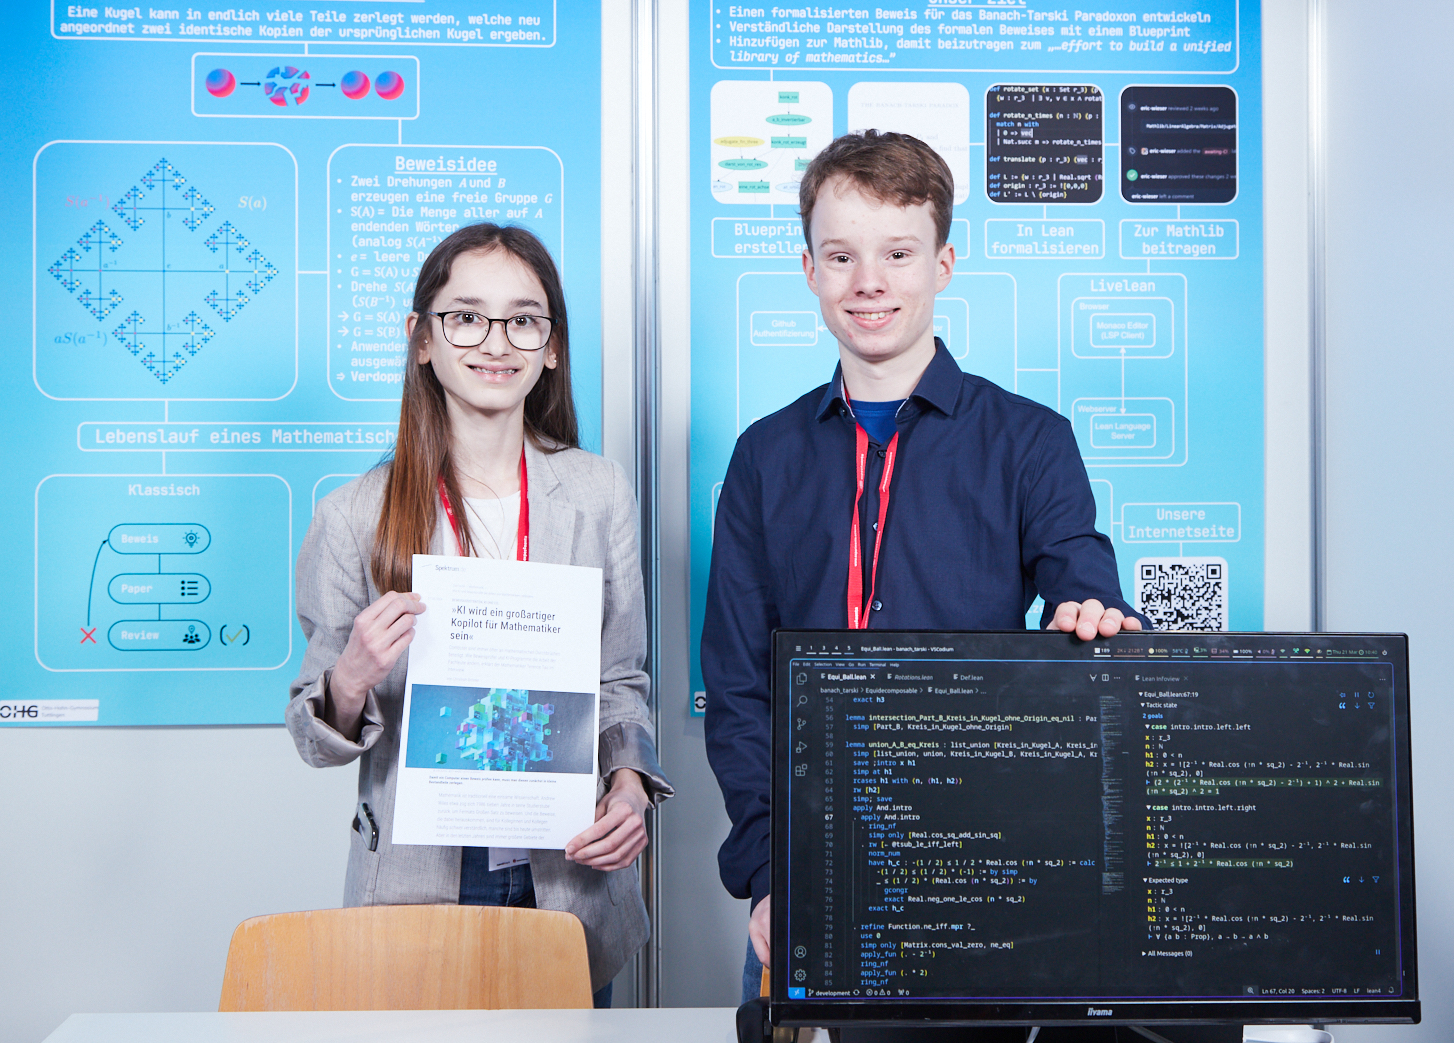
\includegraphics[scale=0.5]{M-07.jpg}

    \end{figure*}
    \begin{center}


        \Large\textsc{Chiara Cimino, Otto-Hahn-Gymnasium Tuttlingen\\Christian Krause, Gymnasium Ochsenhausen}\\\vspace{0.7cm}

        Schülerforschungszentrum Südwürttemberg e.V.\\Standorte Tuttlingen und Ochsenhausen  \vspace{1cm}

        \today

    \end{center}~
    \clearpage

    \section*{Projektübersicht}
    Das Ziel unseres Jugend-forscht-Projekts des letzten Jahres war es, das Banach-Tarski-Paradoxon, welches besagt, dass wir eine Kugel allein durch Zerlegen und Neuanordnen in zwei identische Kugeln duplizieren können, mithilfe des Beweisassistenten Lean zu formalisieren und der Lean-Community zur Verfügung zu stellen. Aber warum ist diese Art der Kugelverdopplung, die ja offensichtlich den Gesetzen der Physik widerspricht, in der Mathematik überhaupt möglich? Wir machten es uns vor dem Hintergrund dieser Frage deshalb zur Aufgabe, die Problematik hinter Banach-Tarski zu beheben und damit das Paradoxon aufzulösen. Da unsere Arbeit über die Jugend-forscht-Phase hinausging, erreichte uns in einem von zahlreichen Gesprächen mit Mathematikern der Hinweis von Fields Medaillen Träger Laurent Lafforgue auf das französische Manuskript von Olivier Leroy \glqq Les intersections cachees dans le paradoxe de Banach-Tarski\grqq. Dieses Manuskript weist auf eine allgemeinere Theorie hin, in der die Problematik hinter Banach-Tarski behoben wird, weshalb wir uns intensiv mit Leroys Arbeit beschäftigten. Da diese nie in einem Journal veröffentlicht und damit auch nie offiziell geprüft wurde, begannen wir, seine Ideen mit anderen Theorien in Verbindung zu setzen und damit das Manuskript zu vervollständigen. Hierfür mussten wir zunächst einige mathematische Definitionen und Lemmata leanen, wobei es uns bereits gelang, einen signifikanten Teil der Lean-Community zur Verfügung zu stellen. Ausgehend davon haben wir bereits das gesamte Manuskript von Leroy in Lean formalisiert und dadurch vervollständigt und verifiziert. Mit Leroys Ansatz ist dann der Satz von Banach-Tarski kein Paradoxon mehr, da mit dieser Theorie die Banach-Tarski-Zerlegung nicht mehr disjunkt wäre.



    \thispagestyle{empty}

    \clearpage
    \tableofcontents
    \listoffigures
    \thispagestyle{empty}

    \clearpage
    \setcounter{page}{1}


    \section{Fachliche Kurzfassung}
    % Als wir letztes Jahr dabei waren, den Satz von Banach-Tarski in Lean zu formalisieren, sind wir an die Grenzen der klassischen Maßtheorie gestoßen. Der Satz von Banach-Tarski besagt nämlich, dass es theoretisch möglich ist, eine Kugel allein durch Zerschneiden und Drehen zu verdoppeln. Das ist möglich, da während des Zerschneidungsprozesses nicht messbare Teilmengen des topologischen Raums erzeugt werden. Auf der Suche nach einer Lösung für dieses Problem sind wir auf ein nie formal veröffentlichtes Manuskript von Olivier Leroy gestoßen, das verspricht das Problem der nicht messbaren Mengen von Banach-Tarski in der Theorie der Lokalen zu lösen. Dabei werden Unterlokalen anstatt von Teilmengen von topologischen Räumen verwendet. Wir haben es uns zur Aufgabe gemacht, die Grundlagen der Lokalen-Theorie und das von Leroy postulierte Maß zu verstehen und in Lean zu verifizieren. Dafür haben wir bereits viele elementare topologische Definitionen (z.B. Inklusion, Schnitt, Vereinigung und Komplement) auf die Unterlokalen übertragen und in Lean formalisiert. Ausgehend davon arbeiten wir daran, zu zeigen, dass die Caratheodory Erweiterung eines Maßes der offenen Unterlokalen auf alle Unterlokalen einige wichtige maßtheorethische Eigenschaften erfüllt. Damit ist der Satz von Banach-Tarski dann kein Paradoxon mehr, da mit dieser neuen Maßtheorie das Verdoppeln einer Kugel in zwei identische Teile nicht mehr möglich ist.
    Wenn man in der klassischen Maßtheorie ein Maß mithilfe der Caratheodory Erweiterung auf die gesamte Potenzmenge erweitert, so besitzt diese Erweiterung im Allgemeinen nicht mehr dieselben nützlichen Eigenschaften wie bspw. die strikte Additivität. Die Folgen sind im Banach-Tarski-Paradoxon zu erkennen, welches eine Kugelverdopplung ermöglicht. Im Zuge dieses Projektes beschäftigen wir uns mit einer Theorie, bei der solche Probleme nicht mehr auftauchen, ohne jedoch die zu messenden Mengen einschränken zu müssen, wobei diese Theorie insbesondere nie in einem mathematischen Journal veröffentlicht wurde. Es handelt sich dabei um die Theorie der Lokale, auf die der französische Mathematiker Olivier Leroy in seinen Notizen aufbaut. Lokale sind dabei intuitiv als die offenen Mengen eines Topologischen Raums zu verstehen, wobei wir nicht mehr fordern, dass das zugrundeliegende geordnete Mengensystem eine Teilmenge der Potenzmenge eines festen gegebenen Raums ist. Daraus resultieren neue Definitionen von Konzepten wie der \glqq Teilmenge\grqq~(Unterobjekte), der Vereinigung und dem Schnitt. Damit lässt sich dann ebenfalls eine Maßtheorie konstruieren, wobei man ein Maß auf einer Lokale ähnlich wie ein klassisches Maß verstehen kann. Betrachtet man allerdings die Caratheodory Erweiterung eines Maßes auf einer Lokale, so erhält man im Gegensatz zu den mangelhaften Eigenschaften der Caratheodory Erweiterung in der klassischen Maßtheorie u. a. eine Reduzibilität und eine strikte Additivität, d. h. die Caratheodory Erweiterung eines Maßes auf einer Lokale bleibt insbesondere ein Maß. Daher erhält man eine bessere Maßtheorie! Da dieses unglaubliche Resultat aber nie formal veröffentlicht und damit peer-reviewed wurde, besteht unsere Arbeit darin, genau das zu tun. Hierfür verwenden wir den mathematischen Beweisassistenten Lean, mit dessen Hilfe wir Ungenauigkeiten und Lücken im Beweis von Leroy aufdecken und beheben konnten und damit den Großteil seiner Theorie bereits in Lean formalisiert haben. Des Weiteren gelang es uns bereits, Teile des von uns formalisierten Beweises in der Mathlib zu veröffentlichen. Dort werden viele bereits in Lean formalisierte Definitionen und Theoreme gespeichert.


    \section{Motivation und Aufgabenstellung}
    \glqq Wir können eine Kugel allein durch Zerschneiden und anschließendem Drehen wieder zu zwei identischen Kopien der Ausgangskugel zusammenfügen, also insgesamt verdoppeln.\grqq~Dass das mit der klassischen Mengenlehre gilt, folgt aus dem Satz von Banach-Tarski \autocite{noauthor_banach-tarski-paradoxon_2024}. Uns erschien diese Aussage anfänglich unglaublich, weshalb wir in unserem Jugend-forscht-Projekt des letzten Jahres den mathematischen Beweis des Banach-Tarski-Paradoxons näher beleuchteten.
    Indem wir den Beweis Stück für Stück durchdrangen, gingen wir automatisch den Weg einer klassischen Verifikation eines mathematischen Papers (siehe Abbildung \ref{Abb1}, linke Spalte). Da der Prozess der menschlichen Kontrolle aber durchaus fehleranfällig ist, stellten wir uns die Frage, ob man diese Fehlbarkeit nicht umgehen könnte. Dabei stießen wir auf den mathematischen Beweisassistenten Lean. Diese auf der gleichnamigen Programmiersprache Lean basierende Software erlaubt es uns, die entsprechenden mathematischen Objekte zu definieren, sowie deren Eigenschaften inkl. Beweis zu formalisieren. Basierend auf Typentheorie überprüft Lean die Standhaftigkeit des Beweises und markiert ggf. Fehler, was das Beweisen erleichtert. Dies bedeutet im Umkehrschluss aber auch, dass Lean den Anspruch einer absoluten mathematischen Korrektheit erheben kann (siehe Abbildung \ref{Abb1}, rechte Spalte). Die Mathlib Community von mittlerweile fast 400 Contributern, zu der wir nun seit einem Jahr gehören, hat bereits über die Hälfte des Grundstudiums der Mathematik, sowie einige sehr fortgeschrittene Konzepte in insgesamt über eine Million Zeilen Code digitalisiert.


    \begin{wrapfigure}{R}{0.48\textwidth}
        \begin{center}
            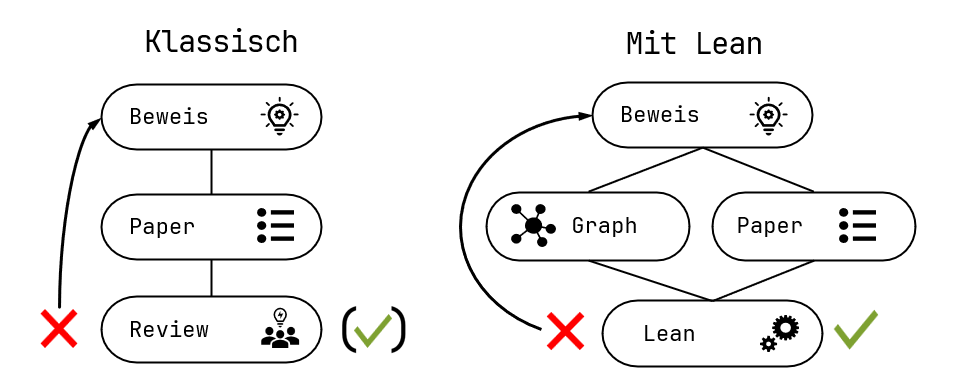
\includegraphics[width=0.48\textwidth]{Formalisierung_Grafik.png}
        \end{center}
        \caption{Verifikation mit bzw. ohne Beweisassistent}
        \label{Abb1}
    \end{wrapfigure}
    \noindent Das ist auch der Grund, weshalb sich Mathematikerinnen und Mathematiker weltweit vernetzen, um weitere Sätze in Lean zu formalisieren. Hier erleben wir eine wunderbare und effektive Zusammenarbeit der Informatik und der Mathematik. \\
    \noindent Je länger wir uns jedoch mit dem Beweis des Satzes von Banach-Tarski beschäftigten, desto öfter kam die Frage auf, warum das Duplizieren einer Kugel allein durch Zerlegung der Ausgangskugel sowie anschließender Translationen und Zusammenfügen der einzelnen Teile in der Mathematik überhaupt erlaubt sein sollte und ob wir diese Defekte in der klassischen Topologie, die dieses Paradoxon überhaupt ermöglichen, nicht mithilfe einer anderen Sichtweise auf die Dinge, genauer gesagt mithilfe einer anderen mathematischen Theorie, beheben könne. Um das aber sauber abgrenzen zu können, ist es essentiell, dass wir die Lücken in der klassischen Maßtheorie identifizieren, was zunächst eine nähere Betrachtung erfordert.


    \section{Kurzer Einblick in die benötigte klassische Maßtheorie}
    Das Grundprinzip der Maßtheorie besteht darin, einer Ansammlung an Mengen eine sinnvolle Größe zuzuordnen. 
    %\rot{Beispiel Landkreisapproximation drin lassen?} Betrachten wir daher als Einführung ein Beispiel: Gegeben sei die Menge aller Rechtecke. Jedem dieser in der Menge enthaltenen Rechtecke wollen wir nun eine Größe bzw. einen sinnvollen Flächeninhalt zuordnen. Solch eine Größe definiert sich in unserem Beispiel als Produkt aus Länge mal Breite des entsprechenden Rechtecks. Durch diese Zuordnung wird ein sog. Maß definiert. 
    Allgemein versteht man unter einem Maß allerdings folgendes:
    % Die Maßtheorie \autocite{noauthor_mastheorie_2023} entstand aus dem Versuch, eine Maßfunktion zu definieren, die jeder Teilmenge eines Raumes eine sinnvolle Größe (z. B. Flächeninhalt) zuordnet. Betrachtet man daher bspw. die Menge aller Rechtecke, so kann mithilfe eines Maßes jedem Rechteck das Produkt aus Länge mal Breite zugeordnet werden. Fordert man allerdings gleichzeitig $\sigma$-Additivität und Bewegungsinvarianz dieser Maßfunktion, so muss man sich auf eine bestimmte Ansammlung von Mengen beschränken, wie Giuseppe Vitali zeigte. Diese Mengen werden als messbar bezeichnet. Auf ihnen können wir daher sog. Maße definieren:

    \begin{definition}
        Sei $X$ eine beliebige Menge  und $\mathcal{M} \subseteq \mathcal P(X)$ eine Teilmenge der Potenzmenge und $\mu:\mathcal{M} \to \overline{\mathbb{R}}$
        eine Abbildung. Man nennt $\mu$ ein Maß, falls folgende Bedingungen erfüllt sind:
        \begin{itemize}
            \item $\mu(\emptyset) = 0$

            \item $\mu(A)$ ist monoton

            \item $\mu$ ist $\sigma$-additiv, insbesondere $\mu(A\cup B)=\mu(A)+\mu(B)-\mu(A\cap B)$ für alle $A, B\in\mathcal{M}$
        \end{itemize}
        Im Folgenden nennen wir $\mathcal M$ die messbaren Mengen.
    \end{definition}
    Wie man erkennen kann, ist ein Maß aber auf ein bestimmtes Mengensystem begrenzt, d. h. Objekte, die nicht in diesem System enthalten sind, kann keine Größe zugeordnet werden. 
    Um diesen Mengen dennoch eine Größe zuzuordnen gibt es die Caratheodory Erweiterung. Sie approximiert die Größe einer beliebigen Menge $Y \subseteq X$ von außen, indem sie den Grenzwert des Maßes aller messbaren Mengen, die $Y$ enthalten, betrachtet: 
\begin{comment}

    %Hat man nun Objekte, die nicht im System vorhanden sind und die eine ähnliche Struktur wie die Elemente des Systems haben, auf dem unser Maß operiert, so ist es naheliegend sich zu fragen, ob man das vorliegende Maß nicht sinnvoll auf diese Objekte erweitern könnte.
    \begin{minipage}{0.5\textwidth}
        Im Beispiel unseres Maßes, welches jedem Rechteck seinen Flächeninhalt zuordnet, entspräche ein solches zu den Rechtecken ähnliches Objekt zum Beispiel der Fläche des Landkreises Tuttlingen. Um nun der Fläche des Landkreises eine sinnvolle Größe zuzuordnen, können wir diesen zunächst einmal mit Rechtecken überdecken. Für die Überdeckung verwenden wir nun immer kleinere Rechtecke und können so den Flächeninhalt des Landkreises approximieren, indem wir den Grenzwert der Summe der Flächeninhalte dieser kleinen Rechtecke betrachten.
    \end{minipage}
    \begin{minipage}{.5\textwidth}
        \centering
        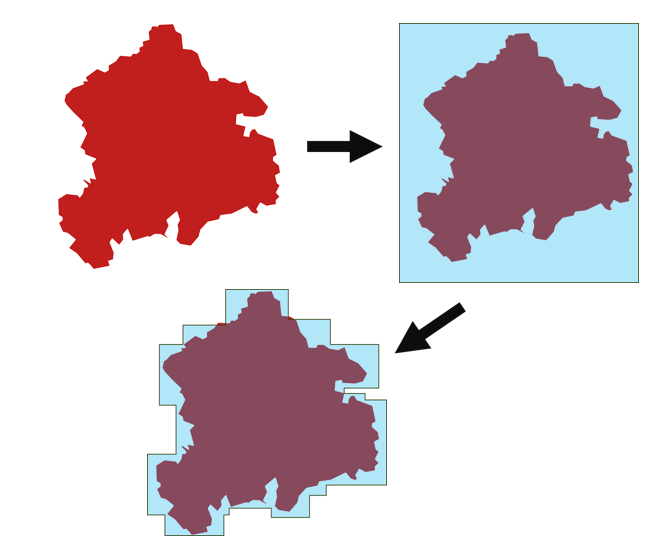
\includegraphics[width=.9\linewidth]{Landkreis approximieren}
        \captionof{figure}{Approximation der Fläche des Landkreises Tuttlingen}
        \label{fig:fläche tut}
    \end{minipage}

    %\noindent Diese Approximation von einer zunächst nicht-messbaren Menge mithilfe von messbaren Mengen und einer anschließenden Grenzwertbetrachtung entspricht allgemein genau dem Prinzip der Caratheodory Erweiterung eines Maßes.
\end{comment}


    \begin{definition}
        Sei $\mu$ ein Maß auf einem Mengensystem $\mathcal{M} \subseteq \mathcal P(X)$. Die Caratheodory Erweiterung des Maßes ist definiert als
        \[\mu^*(Y)=\inf \left\{ \sum_{i=1}^\infty \mu(A_i)~|~A_i\in\mathcal{M},~Y\subset\bigcup_{i=1}^\infty A_i \right\}\] für alle $Y \subseteq X$
    \end{definition}

    Jetzt haben wir zwar einen sinnvollen Größenbegriff für eine größere Ansammlung an Mengen, jedoch ist zu vermerken, dass bei der Caratheodory Erweiterung Eigenschaften wie bspw. die allgemeine strikte Additivität verloren gehen. Dieser Verlust der strikten Additivität spiegelt sich bspw. im Banach-Tarski-Paradoxon wider.
    Dass man somit eine Kugel verdoppeln kann, hat uns ziemlich gestört und wir haben uns gefragt, ob es nicht eine Möglichkeit gibt, dass eine Caratheodory Erweiterung eines Maßes die strikte Additivität des Ausgangsmaßes übernimmt.
    Dabei sind wir auf die Theorie der Lokale gestoßen.

    \section{Die Theorie der Lokale und erste Ergebnisse unserer Arbeit}
    \noindent Unsere Arbeit basiert auf dem Dokument \glqq Théorie de la mesure dans les lieux réguliers\grqq~(1995) \autocite{leroy_theorie_2013}, das behauptet, dass die Caratheodory Erweiterung eines Maßes auf die Unterlokale einer Lokale ein Maß mit guten Eigenschaften (z.B: strikte Additivität) liefert und damit das Banach-Tarski-Paradoxon auflöst.\\
    \noindent Das Problem an diesem Dokument ist allerdings, dass es lediglich aus den Notitzen von Olivier Leroy besteht,
    die nach seinem Tod im Jahr 1996 digitalisiert wurden.
    Daher wurde das Paper auch nie in einem mathematischen Journal veröffentlicht und damit auch nie peer-reviewed (also durch andere Mathematiker kontrolliert).
    Da die Notizen von Leroy zudem teilweise sehr vage formuliert sind, keine Quellenangaben enthalten und mit kleinen
    Fehlern behaftet sind, haben wir es uns zur Aufgabe gemacht, das Dokument zu vervollständigen, in Lean zu formalisieren und damit zu
    verifizieren.
        \end{document}
    \begin{comment}
    \noindent Dafür müssen wir zunächst aber etwas genauer auf die Theorie der Lokale, die eine spezielle Form der
    punktfreien Topologie darstellt, eingehen.
    Eine Lokale \autocite{noauthor_locale_nodate} verhält sich intuitiv wie ein topologischer Raum, der möglicherweise nicht genügend (oder sogar gar keine) Punkte besitzt.
    Stattdessen enthält ein Lokal offene Unterräume. Diese offenen Unterräume können so verstanden werden, dass sie eine
    endliche Menge an Informationen über die (hypothetischen) Punkte beinhalten.
    \begin{example} 
    TODO hier vlt nix sagen und das erst nach def definition von ner Loakale machen
        Example for pointless locale (nicht ganz trivial)
    \end{example}
    %Zum Beispiel gibt es eine Lokale aller
    %Surjektionen von den natürlichen Zahlen auf die reellen Zahlen. Diese Lokale hat offensichtlich keine Punkte, da es
    %keine derartigen Surjektionen gibt, sie enthält jedoch viele nichttriviale offene Teilräume.
    \begin{example}
        Die offenen Unterräume eines Topologischen Raumes bilden eine Lokale. Eine solche Lokale nennt man räumlich oder topologisch.
    \end{example}
    \end{comment}
        \end{document}
    Leroy zeigt nun durch die Anwendung der Theorie der Lokale, dass es möglich ist, das Auswahlaxiom zu verwenden und dennoch sicherzustellen, dass
    alle \glqq Teilmengen\grqq~messbar bleiben. Eine Lokale \autocite{noauthor_locale_nodate} verhält sich intuitiv wie ein topologischer Raum, der möglicherweise nicht genügend (oder sogar gar keine) Punkte besitzt. Leroy verwendet nun Unterlokalen einer Lokale, die als Unterräume fungieren. In diesem Kontext behauptet er, dass die Caratheodory Erweiterung eines Maßes auf die Gesamtheit der Unterlokale immer noch strikt additiv, reduzibel und kommutativ bzgl. Infima ist. Dadurch werden die paradoxen Zerlegungen wie sie bei Banach-Tarski zu finden sind und die in der klassischen Theorie zu nicht messbaren Mengen führen, in der Theorie der Lokale vermieden, da es versteckte Schnittmengen gibt, die in der klassischen Betrachtung nicht sichtbar sind.
\end{document}
    \subsection{Unser Blueprint}
    Ein wesentliches Hilfsmittel, um bei bei der Arbeit in Lean die Übersicht nicht zu verlieren, ist das sogenannte Lean-Blueprint-Tool \autocite{massot_patrickmassotleanblueprint_2025}, das auch in vielen großen Formalisierungsprojekten zum Einsatz kommt.
    Es bietet die Möglichkeit, alle Definitionen und Lemmata für Menschen verständlich zu formulieren und zu dem
    entsprechenden Lean Code zu verlinken. Eine der wichtigsten Funktionen des Lean-Blueprint-Tools ist wohl der
    interaktive Dependency-Graph (siehe Abbildung \ref{fig:test1}). Dieser stellt alle Beziehungen zwischen den Lemmata und Definitionen übersichtlich in einem Graph dar (also welche Lemmata und Definitionen müssen zuerst fertiggestellt werden). Außerdem kann man anhand der Farbe der Knoten erkennen, wie weit die Formalisierung bereits fortgeschritten ist. \\
    Wir haben für unser Projekt einen solchen Blueprint erstellt, der unter folgender Internetadresse veröffentlicht ist: \url{https://bergschaf.github.io/Localic-Caratheodory-Extensions/blueprint/dep_graph_chapter_1.html}.
    \begin{figure}[h]
        \centering
        \begin{minipage}{.4\textwidth}
            \centering
            \includegraphics[width=.9\linewidth]{Screenshot 2025-04-06 162533.png}
            \captionof{figure}{Gesamtansicht des Blueprints}
            \label{fig:test1}
        \end{minipage}%
        \begin{minipage}{.5\textwidth}
            \centering
            \includegraphics[width=1.05\linewidth]{Screenshot 2025-04-06 163215.png}
            \captionof{figure}{Ein Ausschnitt des Blueprints}
            \label{fig:test2}
        \end{minipage}
    \end{figure}
    \begin{itemize}
        \item Im Blueprint werden Definitionen durch Rechtecke und Lemmata durch Ellipsen dargestellt.
        \item Alles, was bereits fertig formalisiert ist, ist in grün dargestellt.
        \item In Lean formalisierte Definitionen und Lemmata, die wir bereits der Mathlib hinzufügen konnten, sind gelb umrandet.
        %\item Eine Definition oder ein Lemma ist blau unterlegt, wenn alle Voraussetzungen bereits formalisiert sind und die Aussage nun bereit für die Formalisierung ist.
        %\item Wenn bei einem Lemma nur der Rand eingefärbt ist, bedeutet dies, dass nur die Aussage (nicht aber der Beweis) formalisiert ist (bzw. bereit für die Formalisierung ist).
        \item Ein Klick auf einen Knoten des Graphs öffnet eine Ansicht, die die entsprechende Aussage/Definition anzeigt.
        \item Das Feld \textit{latex} führt zu der ausführlicheren Beschreibung der Aussage bzw. Definition im Fließtext-Teil des Blueprints.
        \item Über das Feld \textit{lean} gelangt man zu der automatisch generierten Dokumentation des dazugehörigen Lean Codes. In dieser Dokumentation ist zu jedem Abschnitt der entsprechende Quellcode unter \textit{source} verlinkt.
    \end{itemize}
    Da wir bereits alles in Lean verifiziert haben (alle Knoten sind grün), können wir im weiteren Verlauf der Langfassung für viele Lemmata die schriftlichen Beweise weglassen, um für Übersichtlichkeit zu sorgen.
    Die Definitionen und Beweise, die wir in Lean verifiziert haben oder die bereits in der Mathlib enthalten sind, sind folgendermaßen gekennzeichnet:
    \leanok{Measure} bzw. \mathlibok{Nucleus}.
    Die Links zu unserer Lean-Dokumentation bzw. zu der Mathlib-Dokumentation sind im Quellenverzeichniss enthalten.
\end{document}
    \subsection{Elementare Definitionen und Lemmata der Theorie der Lokale}\label{Einführung Lokale}
    Nun wollen wir aber die benötigte Theorie der Lokale besser verstehen. Allgemein besteht eine Lokale $E$ aus einer
    teilgeordneten Menge $O(E)$ (mit einer Ordnungsrelation $\le$), die die Eigenschaften eines Frames \mathlibok{Order.Frame} (bzw. einer
    vollständigen Heyting Algebra \cite{noauthor_heyting-algebra_2024}) erfüllt.
    \begin{definition}
        Eine Lokale $E$ besteht aus einem Paar $(O(E), \le)$, wobei $O(E)$ eine partiell geordnete Menge mit der Ordnungsrelation $\le$
        bezeichnet, die die Eigenschaften eines Frames erfüllt:\\
         Wir verwenden im Folgenden die Notation $\bigvee^E$ und $\bigwedge^E$ um zu kennzeichnen, dass es sich um Suprema bzw. Infima der offenen Elemente der Lokalen $O(E)$ handelt. (Das selbe gilt für $\top^E$ und $\bot^E$.)
        \begin{itemize}
            \item Es existiert ein kleinstes Element $\bot^E$ und ein größtes Element $\top^E$.
            \item Jede Familie $(V_i)$ von Elementen aus $O(E)$ besitzt ein Supremum (genannt Vereinigung), welches mit $\bigvee^{E}_i V_i$ bezeichnet wird.
            \item Jede endliche Familie $(V_i)$ von Elementen aus $O(E)$ besitzt ein Infimum (genannt Schnitt), welches mit $\bigwedge^{E}_i V_i$ bezeichnet wird.
            \item Für jede Familie $(V_i)$ von Elementen aus $O(E)$ und für ein beliebiges $W\in O(E)$ gilt \\
            $$W\wedge \bigvee^{E}_i V_i = \bigvee^{E}_i (W\wedge V_i)$$.
        \end{itemize}
    \end{definition}
   
    Man kann daher erkennen, dass die Definition einer Lokale fast der Definition eines Topologischen Raums entspricht. Der einzige Unterschied besteht dabei darin, dass wir nun nicht mehr fordern, dass das Mengensystem $O(E)$ Teilmenge der Potenzmenge $\mathcal{P}(X)$ einer Ausgangsmenge $X$ ist.
    \begin{example} % TODO entweder das Beispiel hier oder gleich oben?
        \label{bsp:offeneMengen}
        Die offenen Mengen $O(E)$ eines Topologischen Raumes $E$ bilden mit der Inklusion als Ordnungsrelation eine
        Lokale \mathlibok{TopologicalSpace.Opens.instFrame}. Eine solche Lokale nennt man topologisch.
    \end{example}
            \end{document}
